\subsection{Focus on the user}
A large part of the objective outlined in section 3.1, design, is defined by the service that we want to offer
to the user, since this is our final client and to whom we intend to help. \\


We must be aware of the needs that users show in combination with market deficiencies since
It will help us to know what the demand or the hole that is not covered may be.
Whether our target audience is unique, that is, take all types of users equally, considering the
average user, as for a characteristic user, we should know the homogeneous characteristics of our group.

Therefore we need a current study on the psychological, social and economic level of the target group, to discover, not only
the needs, but also the wishes, that you would like to have and your demands, that you want.

Once the users have access to the data as we provide them, it is important to have a feedback,
It would be ideal to be able to perform an analysis of user behavior to see their guidelines regarding the data obtained.
\subsubsection{How to solve it} 
Define what type of users is intended. Study both its characteristics and the situation of the
market.
Use a mechanism that helps us obtain a feedback, either by a system of points, test or
an automatic mechanism that allows knowing the behavior of the user. We can also choose the combination of both
options

\subsubsection{How we solve it. Aire Guru} 
Air Guru is aimed at the entire population, so we will take into account when implementing it that the information should
show in a simple way, in addition to complete. In addition, we pay special attention to users who may have a
disease or medical condition influenced by air pollution.
During the market study, we realized that many of them offered air pollution in real time, but
We could see the following deficiencies:
\begin{itemize}
    \item Obsolete measurements. Measurements need to be taken regularly, since there can be huge differences
    between pollution levels at different times of the day.
    \item Limited geographic coverage. The data must cover a reasonable proportion of areas that people spend significant time in.
    \item Insufficiently granular measurements. Measurements must be at a reasonably fine level of granularity. One single measurement for an entire city is not useful.
    \item Poor presentation. Often the information is presented in an uninterpreted form, making it difficult for users to visualize, especially in a geographic sense.
    \item Poor discrimination and interpretation. Many tools show individual values as a number or a colour. This information is not
    enough for the user to take control of their exposure. Such visualizations are not really compelling. 
    \item Exposicion a la polucion de una forma personalizada. Nos interesa saber a que nivel de polucion estamos expuesto
    a lo largo del tiempo, no de forma puntual.
    \item Necesidad de utilizar complicated devices para monitorizar la exposicion. Nuestro objetivo es facilitar la informacion a los 
    usuarios con el minimo de complicaciones posibles.
    \item Sin informacion dedicada por condicion medica.
\end{itemize}

Once implemented, we tested the tool with 14 users. Our tool integrates Google Analytis that allows us to know the
user behavior, how many pages they access, how long and how long they stay in it. Also, after the test,
A survey was conducted to measure not only the level of satisfaction, but also to verify the utility and if it had achieved the objective.
\begin{figure}[ht]
    \centering
   \subfigure[Aire Guru Form]
    {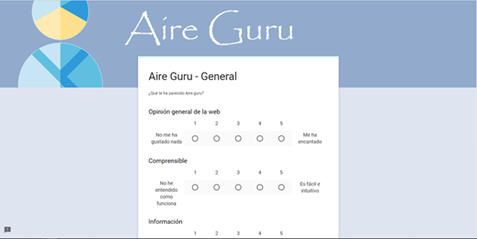
\includegraphics[width=5.5cm  ]{form}}
    \hfill
    \subfigure [Google Analytics]
       { 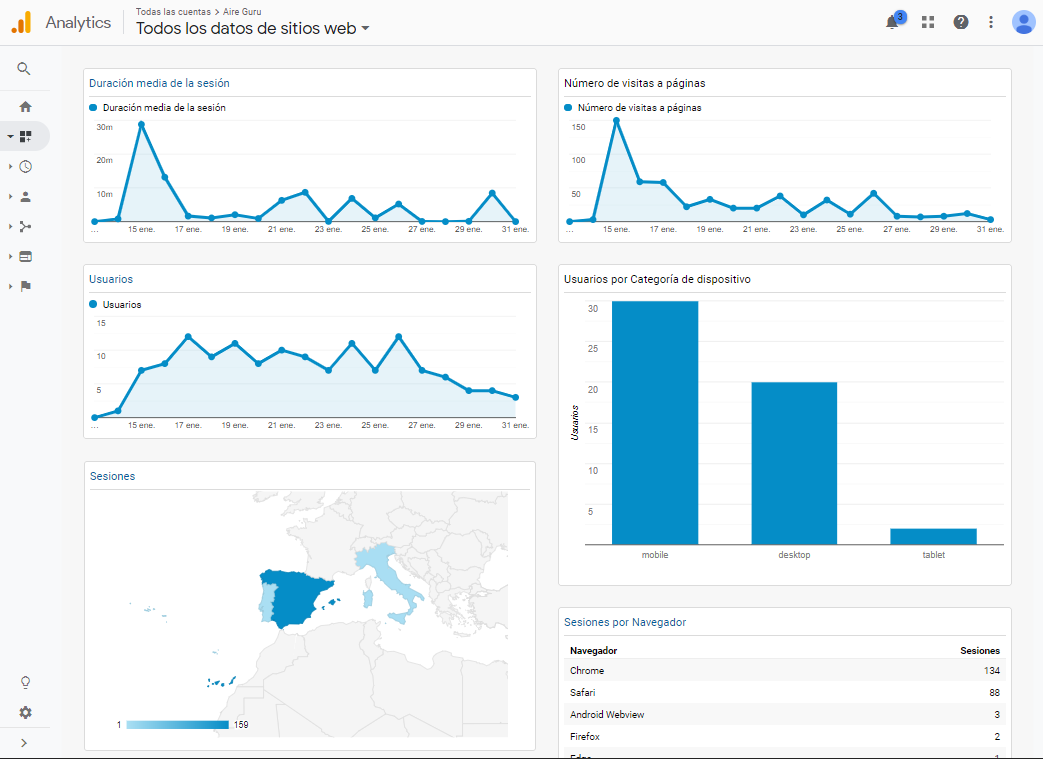
\includegraphics[width=5.5cm]{googleAnalytics}}
  
  \caption{User Feedback}
    \end{figure}
 
\elsparagraph{Evaluation}  
\begin{itemize}
    \done The market study made us clearly see the shortcomings that exist in current applications.
    \done The survey gave us very positive evaluations regarding the use, understanding and information reported.
    \done Users were told that thanks to Aire Guru they had discovered that they had a medical condition that could be affected by
         air pollution

\end{itemize}
 

\newpage